\documentclass[lettersize,journal]{IEEEtran}
\usepackage{amsmath,amsfonts}
\usepackage{algorithmic}
\usepackage{array}
\usepackage[caption=false,font=normalsize,labelfont=sf,textfont=sf]{subfig}
\usepackage{textcomp}
\usepackage{stfloats}
\usepackage{url}
\usepackage{verbatim}
\usepackage{graphicx}
\usepackage{cite}
\usepackage{balance}
\usepackage[acronym]{glossaries}
\usepackage{cleveref}
\usepackage{subcaption}

\makeglossaries

% Define the acronym
\newacronym{adam}{ADAM}{Adaptive Moment Estimation}

\begin{document}

\title{Development and Comparative Evaluation of UNet Architectures for Image Segmentation On Annotated Brain Tumor MRI Scans}

\author{Jakob Müller, Konrad Wolf
\thanks{This work is created as a semester thesis in Computer Vision at the Cooperative State University Baden-Württemberg Center for Advanced Studies at Heilbronn. The opinions expressed here are entirely that of the author. No warranty is expressed or implied. User assumes all risk.}}
\markboth{Computer Vision, Prof. Dr. Matthias Drüppel, July~2024}%
{Development and Comparative Evaluation of Neural Network Architectures for Image Segmentation On Annotated Brain Tumor MRI Scans}



\maketitle



\begin{abstract}
  In the field of medical imaging, brain tumor segmentation remains one of the most important tasks, crucial for accurate diagnosis and treatment of cancer, one of the worst diseases we face today. With different approaches to this problem already existing, we try training our own models for this challenge, comparing two different architectures. In this paper we use a dataset of brain scans showing tumors, that we describe in detail. Our models are based on the same U-Net architecture with one model utilizing a pretrained ResNet50 as the encoder. Both models are then trained under the same initial conditions and compared trough the same metrics. We find that during training the model without ResNet tends to perform better for tumor segmentation but exhibits overfitting tendencies, possibly benefitting from hyperparameter tuning or data augmentation. In contrast, the pre-trained model demonstrates more stable performance, though further fine-tuning of its pre-trained weights could potentially improve results further.
\end{abstract}



\begin{IEEEkeywords}
Computer Vision, Image Segmentation, UNet, ResNet, Transfer Learning, Comparative Evaluation.
\end{IEEEkeywords}


\section{Introduction}
\IEEEPARstart{I}{n} the field of medical imaging, brain tumor segmentation remains one of the most important tasks, crucial for accurate diagnosis and treatment of cancer, one of the worst diseases we face today. 

The objective of this research is to develop and evaluate various models for the segmentation of brain tumors using a dataset of annotated brain MRI scans. Specifically, the study compares three neural network architectures based on quantitative performance metrics, qualitative performance metrics, and compute resource metrics. The goal is to assess each model's segmentation accuracy, viability, and computational efficiency, thereby determining the most effective and resource-efficient approach for brain tumor segmentation.

The goal is to develop and systematically evaluate multiple neural network architectures for the segmentation of brain tumors using annotated MRI datasets by a comprehensive comparison of the models based on quantitative segmentation accuracy metrics and qualitative performance analysis to identify the most effective and efficient approach for brain tumor segmentation.

This work answers how different neural network architectures perform in terms of segmentation accuracy and qualitative assessmen%, and computational efficiency 
t when applied to brain tumor segmentation using annotated MRI datasets. Specifically, we will compare a self-designed UNet that was trained entirely new on this dataset with a UNet using a pretrained ResNet50 backbone.

Therfore we evaluate our results based on the following hypotheses, limited on the given data set and the use case for tumor segmentation:
\begin{enumerate}
  \item New-trained U-Nets and UNets combining a pre-trained and ResNet50 backnone with a custom head can achieve valuable performance in brain tumor segmentation.
  \item The application of transfer learning using a combination of a pre-trained ResNet50 based backbone and a UNet head in one model improves segmentation performance comparing to an self-designed U-Net model with the same head and the double amount of parameters in the ResNet50 backbone.
\end{enumerate}




\section{Related Work}
Image segmentation for tumor detection is a critical area of research in medical imaging, spanning numerous publications. With this paragraph we want to examine relevant, existing methods and architectures in this field of image processing relevant to our work.

In their systematic analysis Shaik et al. \cite{10073734} name different methodologies for medical image segmentation, like SegNeXt \cite{guo2022segnextrethinkingconvolutionalattention} introduced by Meng-Hao Guo et al. that is based on a Convolutional Neural Network (CNN) architecture. CNNs are a class of deep learning architecture and are primarily designed for image processing like classification, object detection, or segmentation. They consist of multiple layers, including convolutional layers, pooling layers, and fully connected layers. Convolutional layers apply multiple filters that move over the input image and calculate a scalar product out of the image section and their weights, creating feature maps that capture features like edges. Pooling layers reduce the dimensions of these feature maps and fully connected layers integrate features to make final predictions. \cite{oshea2015introductionconvolutionalneuralnetworks}

Shaik et al. also present transformer-based models, like TransUNet introduced by Hatamizadeh et al. These architectures use a so-called self-attention algorithm, that determines the importance of different image sections relative to each other, thereby capturing context across the entire image, thus enhancing segmentation performance. \cite{hatamizadeh2021unetrtransformers3dmedical}

Finally, Wacker et al. propose the use of transfer learning for tumor segmentation by implementing a pretrained ResNet34 as the encoder of a U-Net, similar to our approach. However, while Wacker et al. focus on performance and compare the same architecture with and without pretraining, we compare two U-Nets with the same decoder architecture but different encoders. For that they use different output modes of MRI scans as input, whereas we use RGB images. Additionally, they employ Multiple Dice Loss as the loss function and the ADAM optimizer with a learning rate of 0.001. To address low-resolution examples in the test set, they use image processing techniques to prepare the model. With that they are able to demonstrate that a U-Net with a ResNet encoder pretrained on the ImageNet dataset yields better performance for tumor segmentation.
\cite{wacker2020transferlearningbraintumor}


\section[Methods]{Dataset}
The data set used for this work is the \textit{Brain Tumor Image DataSet: Semantic Segmentation} \cite{darabi2024BrainTumorImageDataSet}, sourced from the machine learning platform Kaggle. The dataset consists of 2,146 images showing grayscale MRT scans of brains affected by tumors. We chose this dataset for its thorough documentation, clean data, large sample size and annotations that allow training for segmentation. Each pixel of the images is part of either two classes: Non-Tumor (Class 0) or Tumor (Class 1). The tumors are segmented using the COCO segmentation format, where a .json file contains height, width and coordinates of bounding boxes covering the tumor area. 

The dataset as it is given is already preprocessed through automated orientation of pixel data, resized to 640x640 image format and divided into the following three subsets:

\begin{itemize}
  \item Training set with 1502 images (70 \% of the dataset)
  \item Validation set with 429 images (20 \% of the dataset)
  \item Test set with 215 images (10 \% of the dataset)
\end{itemize}

\begin{figure*}[h]
  \centering
  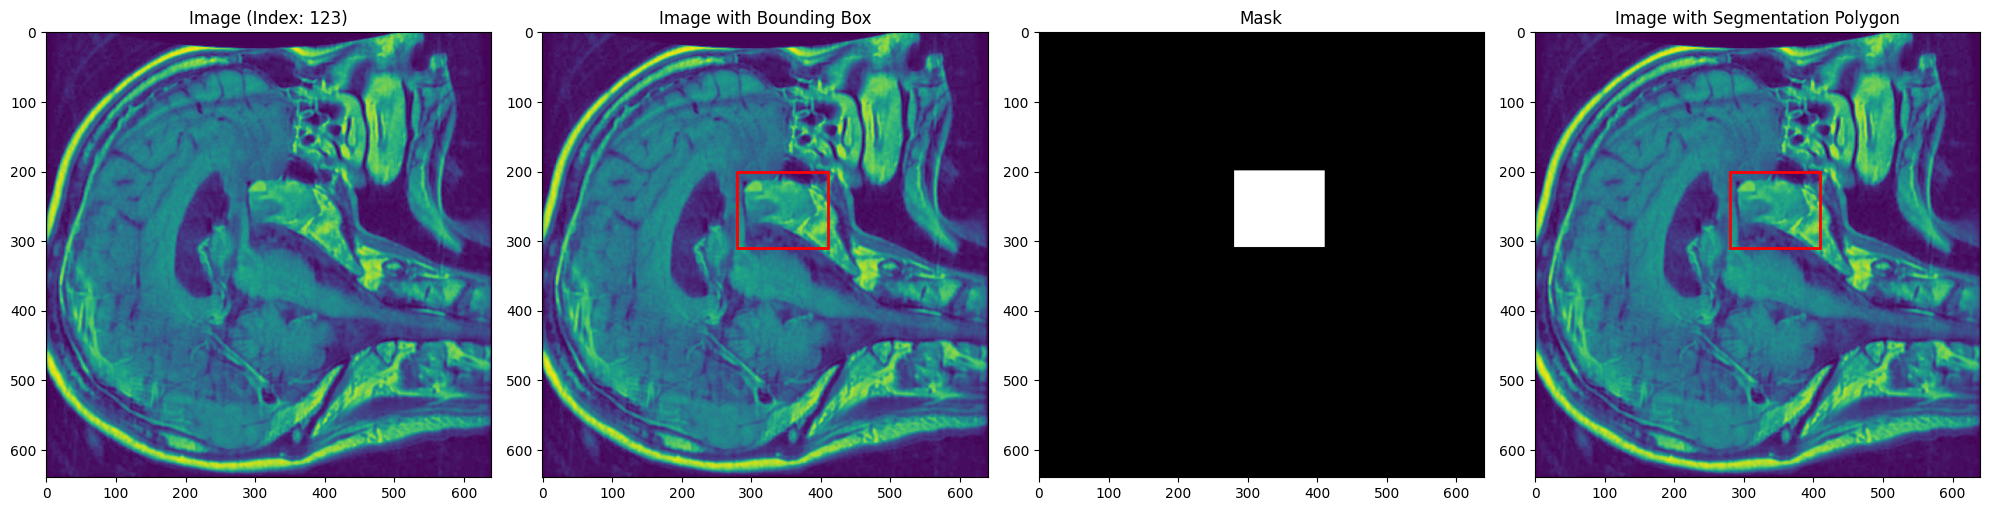
\includegraphics[width=\textwidth]{images/du_image_and_mask.png}
  \caption{Plot of a sample image from the data set, the image with bounding box, the corresponding mask and the visualization of the polygon to show that the polygon does not contain any further useful information compared to the bounding box.}
  \label{fig:da_image_and_mask}
\end{figure*}

\section[Methods]{Methods}
%( Method, Approach** (incl. theory), Development method (data, model architecture, hyperparameters, ...) )

\subsection{Data Preparation and Understanding}
For preprocessing, all images were scaled down to 256x256 pixels, reducing computational load and allowing for faster training while maintaining sufficient detail. Furthermore, the images were normalized, ensuring appropriate scaling with the goal of improving model performance. Given the already substantial size of our dataset, no additional preprocessing or image augmentation was applied to reduce training time.
Finally, the data from the .json annotation file representing bounding boxes is used to generate masks sized 256x256 pixels with one channel. In these masks, pixel values of 1 correspond to tumor regions in the bounding boxes and pixel values of 0 represent non-tumor regions. An example for preprocessed images and the generated masks is shown in \cref{fig:da_image_and_mask}.

Next we compared the training, validation, and test set. For that, we started by investigating the distribution of pixel values after normalization to identify differences between the image quality of the sets. The histograms of the pixel values %\cref{fig:du_histograms} 
show a similar distribution for all three sets, only adjusting the size of the axes accompanying the size of the set, suggesting no major differences between the images.

% \begin{figure*}[h]
%   \centering
%   \subfloat{\label{fig:image1}%
%       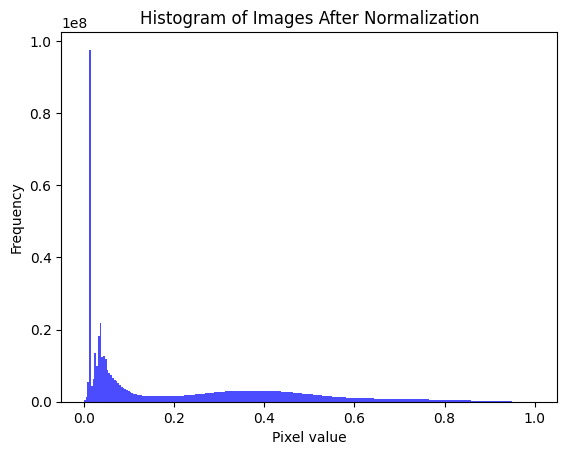
\includegraphics[width=0.3\textwidth]{images/du_histogram_trainingset.png}} \quad
%   \subfloat{\label{fig:image2}%
%       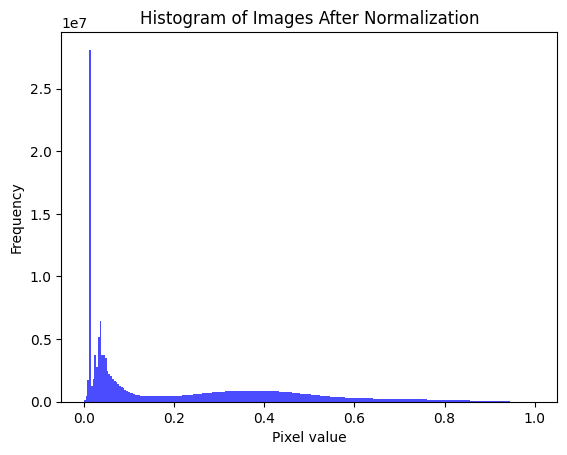
\includegraphics[width=0.3\textwidth]{images/du_histogram_validationset.png}} \quad
%   \subfloat{\label{fig:image3}%
%       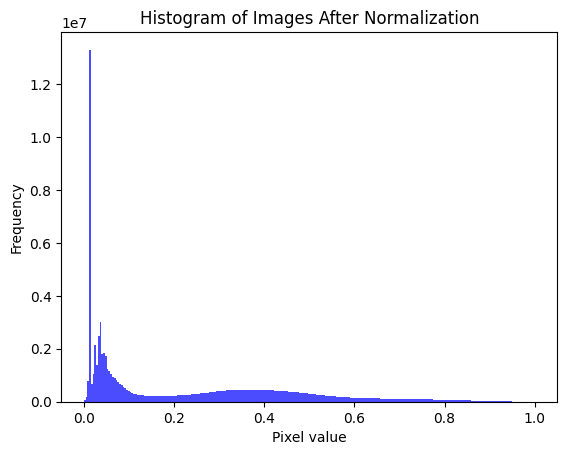
\includegraphics[width=0.3\textwidth]{images/du_histogram_testset.png}}
%   \caption{Histograms of pixel values for training set, validation set, and testset (from left to right).}
%   \label{fig:du_histograms}
% \end{figure*}

To identify difficulties in training, we also compared tumor sizes, shapes, and position with histograms and heatmaps for the centers of the bounding boxes. With average tumor sizes of 14965 pixels for the training set, 15015 pixels for the validation set and 14969 pixels for the test set, the average tumor size does not differentiate significantly between sets, accounting for about 3.63 \% of the total image area. We could also find no major differences in the plotted distribution of the tumor sizes, apart from the training set containing a small number of large tumors sized 100000 pixels and above.

In addition to tumor sizing, we also compared the shape of the tumors. Here the plots of the training and validation set show no significant differences with the distributions both peaking at an aspect ratio of about 1, meaning most tumors are close to square shaped. On the contrary the test set exhibits a slightly more even distribution of differently shaped rectangular tumors.

Finally, we compared the tumor positions between the sets using heatmaps but could not locate any significant differences here either. Therefore, we conclude that the training or performance will not be affected by differences between the training, validation, or test set. 

\begin{figure*}[h]
  \centering
  \subfloat{\label{fig:image1}%
      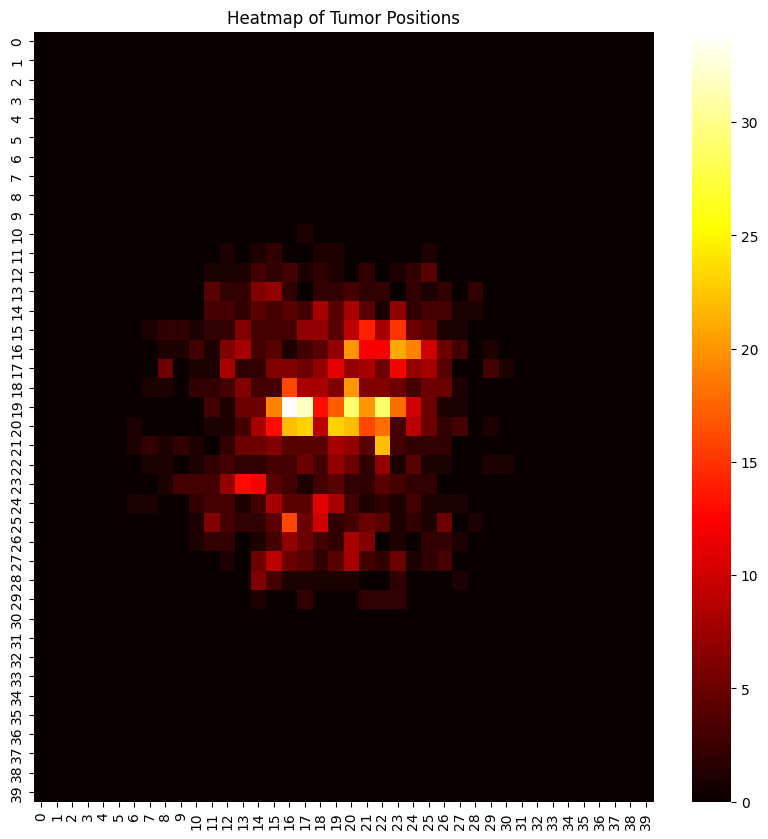
\includegraphics[width=0.3\textwidth]{images/da_trainingset_heatmap.png}} \quad
  \subfloat{\label{fig:image2}%
      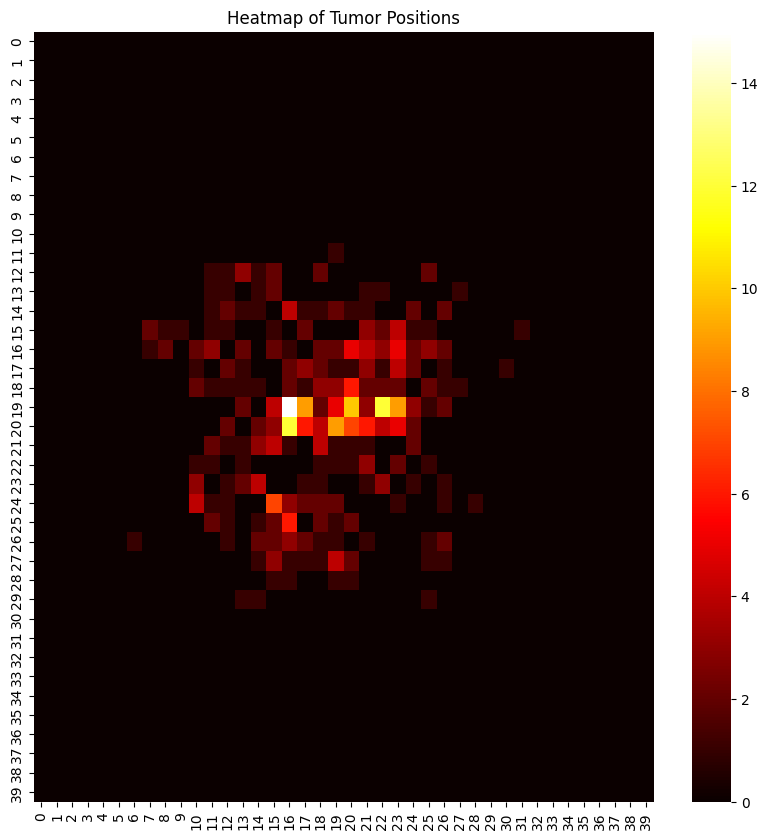
\includegraphics[width=0.3\textwidth]{images/da_validationset_heatmap.png}} \quad
  \subfloat{\label{fig:image3}%
      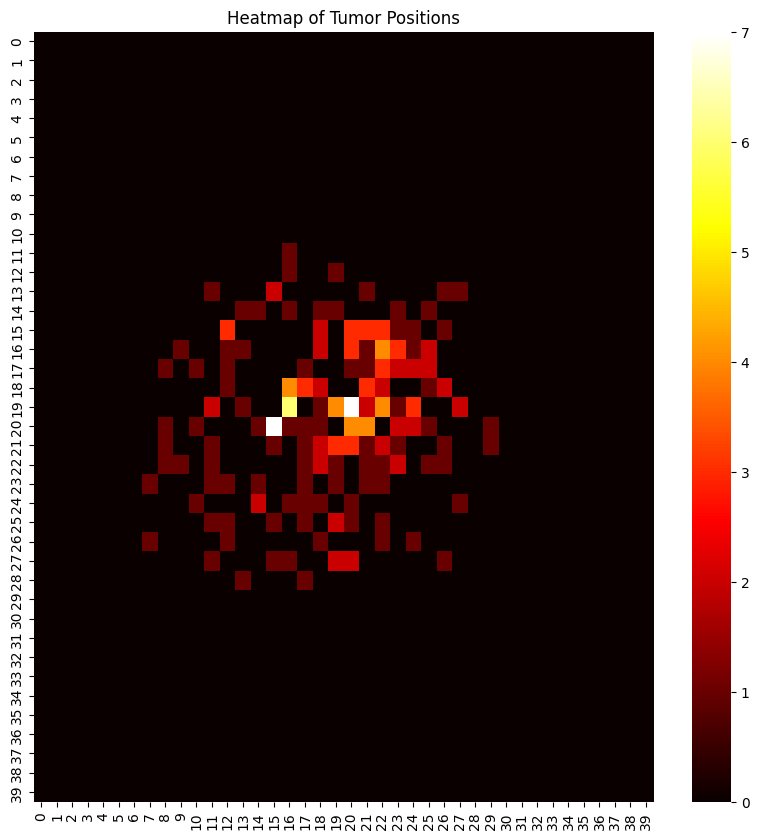
\includegraphics[width=0.3\textwidth]{images/da_testset_heatmap.png}}
  \caption{Heatmap of the positions of bounding box centers for training, validation and test set.}
  \label{fig:da_heatmaps}
\end{figure*}

In conclusion of the data analysis with the described quanitative analysis and further qualitative visualizations of outliers in the distributions of size and shape we find that the split of the data in test, validation and test set is valid to use in this partition in model training and evaluation.

\subsection{Modeling}
Our models are based on the UNET-Architecture, first introduced by Ronneberger et al. in 2015.\cite[text]{ronneberger2015unetconvolutionalnetworksbiomedical}

\begin{figure*}[h]
  \centering
  \subfloat{\label{fig:image5}%
      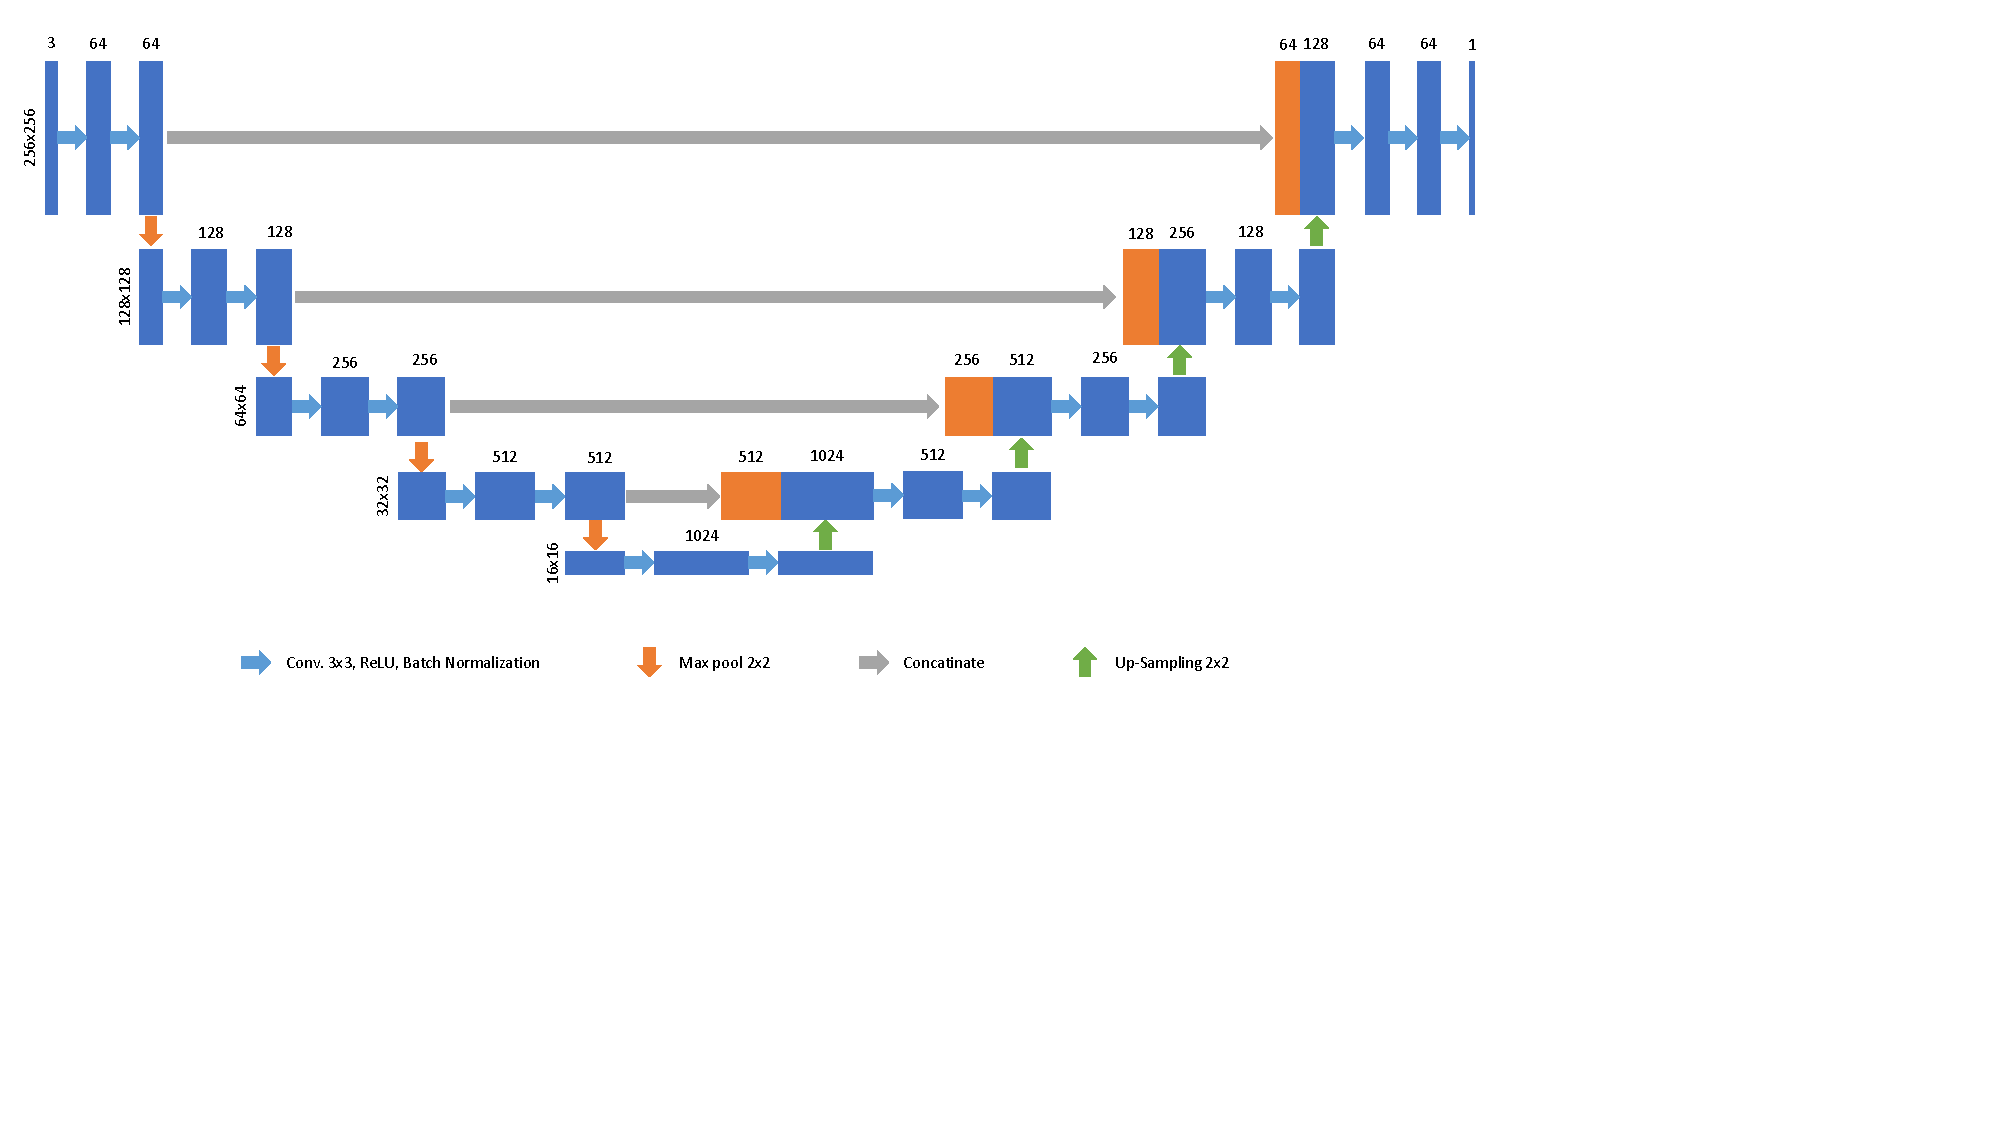
\includegraphics[width=0.45\textwidth]{images/Selfdesigned_unet.pdf}} \quad
  \subfloat{\label{fig:image6}%
      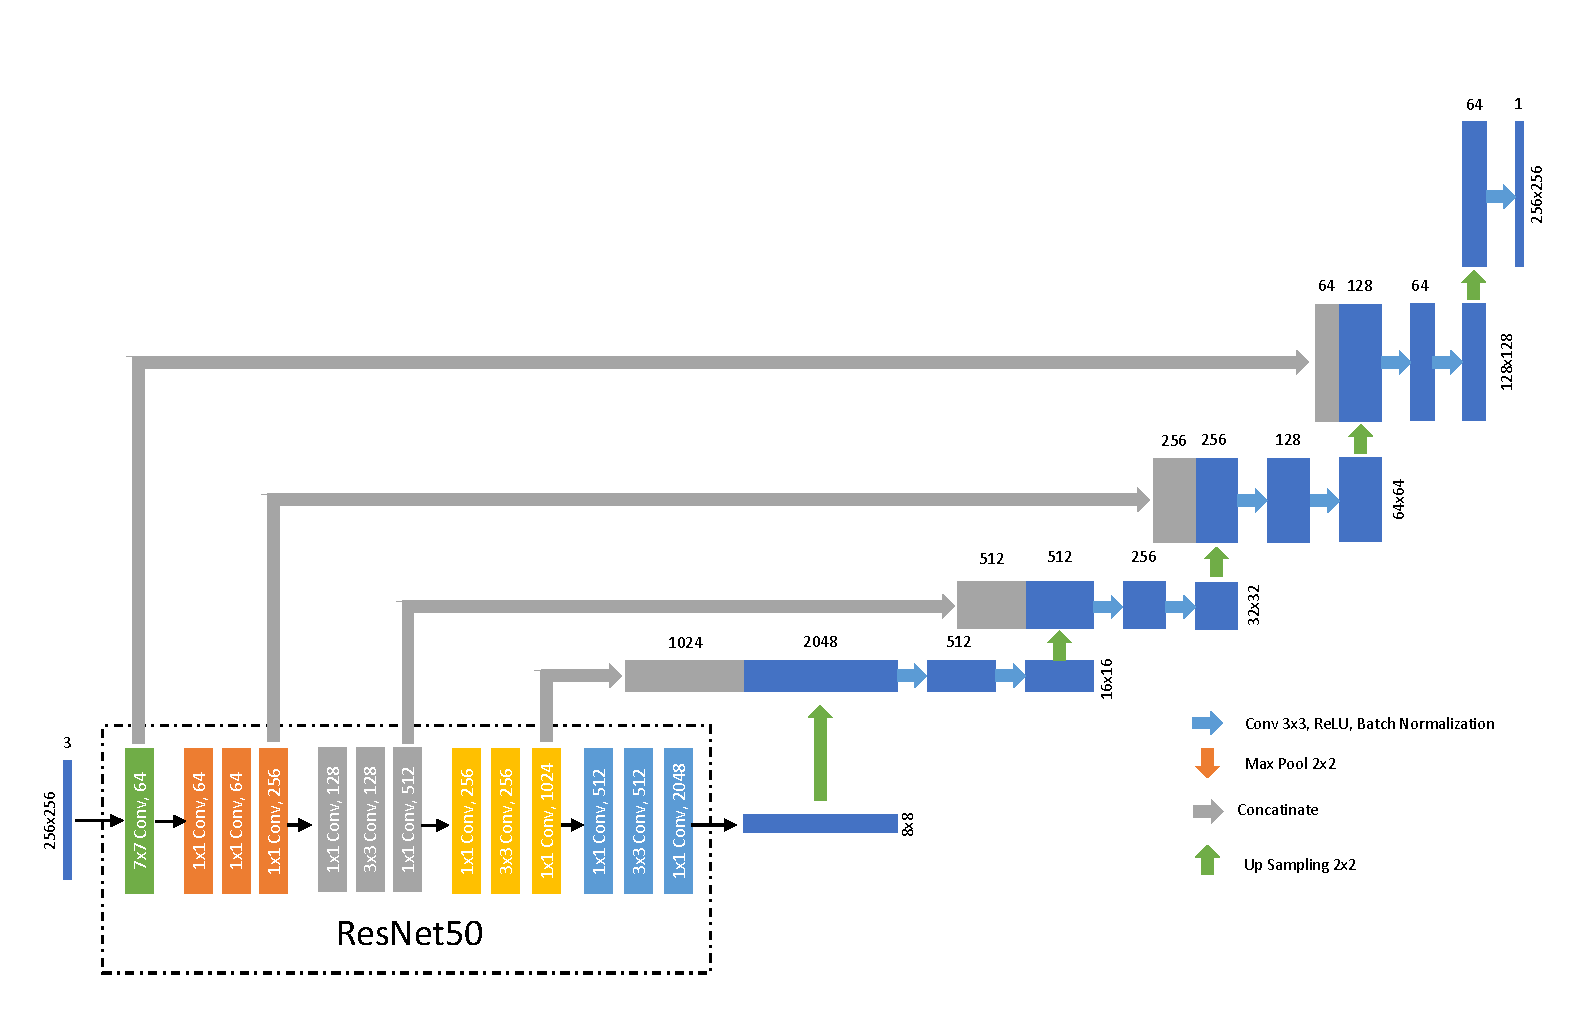
\includegraphics[width=0.45\textwidth]{images/Pretrained_unet-cropped.pdf}}
  \caption{Model architectures of the self-designed UNet and the UNet with pre-trained ResNet50 backbone}
  \label{fig:models}
\end{figure*}
 
In general UNET consists of a symmetrical encoder and a decoder. The decoder downscales images and extracts features by repeatedly applying two 3x3 convolutions with ReLU activation functions, followed by a 2x2 max pooling layer. Here the image dimension is halved while the number of channels is doubled. The decoder first applies upsampling and a 2x2 convolution, halving the number of channels. The result is then concatenated with the output of the corresponding encoder layer. Finally, two 3x3 convolution operations with ReLU activation functions are conducted. These decoder steps are repeated for each encoder step until a final 1x1 convolution reduces the number of channels depending on the number of classes.
 
For our self-designed model we additionally apply batch normalization to the 3x3 convolutions to ensure appropriate scaling. Furthermore, we added padding to maintain a consistent resolution allowing for a straightforward architecture. This way our encoder progressively reduces the 256x256 input resolution of down to 16x16 while increasing the number of channels from 3 input channels to 64 and then to 1024. Our decoder then restores the resolution back up to 256x256, while decreasing the number of channels from 1024 to 64 and finally 1, corresponding to the binary mask.

We use ResNet50 \cite{he2015deepresiduallearningimage} as the encoder of our pretrained UNET for its availability of pre-trained models and proven performance in image processing tasks. To account for the different output resolution of 8x8 with 2048 channels generated by the ResNet50 encoder we added one more layer to the decoder, that upsamples the output to a resolution of 256x256 pixels and reduces the number of channels to 1. Otherwise, the operations performed are the same, with the different upsampling results now being concatenated with the output of the corresponding ResNet50 stage.

To allow a fair comparison we use \gls{adam} introduced by Kingma and Ba in 2014 \cite{kingma2017adammethodstochasticoptimization} for the optimization of both our models as it is proven as an effecitve optimizer in computer vision tasks including image segmentation as well as other machine learning applications. 

As loss function we use binary cross-entropy which computes the loss between a binary true label and a predicted probability. It is defined through the following function with \( y \) being the true label and \( \hat{y} \) the predicted probability:

\begin{equation}
{L} = - \left( y \log(\hat{y}) + (1 - y) \log(1 - \hat{y}) \right)
\end{equation}

\subsection{Training}
For training we started with the ADAM default learning rate of 0.001. As batch size we set 32 because it caused a CPU utilization of around 80 \%. 25 epochs with a training time of around eight hours allowed for overnight training, which is why this number was chosen. Furthermore, we defined a callback reducing the learning rate by a factor of 10 after 3 epochs of no loss improvement to yield better results. Hyperparameters were kept the same for both models to allow for a fair comparison. For monitoring training performance we tracked the following metrics:

\begin{itemize}
  \item Loss
  \item Precision (ratio of true positive examples to all examples that were classified as positive)
  \item Recall (ratio of true positive examples to all true examples), more important because it tracks how many of the tumor area was found
  \item Binary Intersection over Union (ratio of the intersection of predicted and actual tumor area to the union of the predicted and actual tumor area)
\end{itemize}


\subsection{Evaluation}
In alignment to the definitions above we used the following formulas to calculate the evaluation metrics of our models with \( y_i \) and \( \hat{y}_i \) representing the actual and predicted values for the \(i\)-th pixel, respectively, and the total number of pixels denoted by \( N \):
\begin{itemize}
  \item \textbf{Accuracy} is the ratio of correctly predicted pixels to the total number of pixels:
  \begin{equation}
  \text{Accuracy} = \frac{1}{N} \sum_{i=1}^{N} \left( y_i \hat{y}_i + (1 - y_i) (1 - \hat{y}_i) \right)
  \end{equation}
  
  \item \textbf{Recall} is the ratio of true positives to the sum of true positives and false negatives:
  \begin{equation}
  \text{Recall} = \frac{\sum_{i=1}^{N} (y_i \hat{y}_i)}{\sum_{i=1}^{N} y_i}
  \end{equation}
  
  \item \textbf{Precision} is the ratio of true positives to the sum of true positives and false positives:
  \begin{equation}
  \text{Precision} = \frac{\sum_{i=1}^{N} (y_i \hat{y}_i)}{\sum_{i=1}^{N} \hat{y}_i}
  \end{equation}
  
  \item \textbf{Intersection over Union (IoU)} is the ratio of the intersection of the predicted and actual masks to their union:
  \begin{equation}
  \text{IoU} = \frac{\sum_{i=1}^{N} (y_i \hat{y}_i)}{\sum_{i=1}^{N} \left( y_i + \hat{y}_i - y_i \hat{y}_i \right)}
  \end{equation}
\end{itemize}

To calculate the metrics we used the direct outputs of the networks representing the probability of each pixel to depict a tumor. No thresholds were applied for the reason that the outputs are in fact most likely to be used as probabilities and as an overlay over MRI Scans and therefore this is nearest to practical use of the models. Moreover, many thresholds had to be evaluated against each other while loosing information by applying the thresholds.  

The metrics are calculated for each test sample and visualized in a histogram with the mean value over the whole test set. In addition to this quantitative evaluation, we did a qualitative evaluation of each model by visualizing samples from the upper and lower quartile of the distribution of each metric.


\section[Results]{Results}

\subsection{Data Exploration Results}

\subsection{Training Results}

\subsubsection{\textbf{Loss}}
For the loss we did not plot the first two epochs to avoid high initial loss values, making smaller changes in later epochs more visible. The training loss of our self-designed UNET (blue) starts low and steadily decreases. Compared to that, the validation loss (red) starts higher and fluctuates more strongly, while still generally trending downward, showing good generalization despite some instability. Both training and validation losses do not seem to have fully converged yet, indicating a possible benefit from longer training. In contrast, the training (green) and validation (purple) losses of our pre-trained model remain more stable and converge more quickly towards a similar higher value, indicating effective generalization from pre-trained features with less overfitting but also worse performance overall compared to our self-designed UNET.

\subsubsection{\textbf{Precision}}
The training precision of our self-designed model (blue) steadily improves throughout the epochs without fully converging, while the training precision of the pre-trained model (green) follows a similar trend but converges earlier to a lower value. The validation precision of the self-designed model (red) shows a steep upward trend after the seventh epoch with some fluctuation, whereas the pre-trained model's validation precision (purple line) starts increasing earlier but exhibits stronger fluctuation. Both models appear to slightly overfit, with the self-designed UNET demonstrating higher precision in its predictions of tumors.


\subsubsection{\textbf{Recall}}
The training recall of the self-designed model (blue line) improves consistently, while the validation recall of the self-designed model (red line) varies but trends upward. Here, the difference between training and validation recall again suggests overfitting. The training recall of the pre-trained model (green line) converges earlier than that of the self-designed model, while the validation recall (purple line) shows even stronger fluctuation. The peak in epoch 7 is accompanied by a drop in precision, suggesting that the model is identifying large areas as tumors during training, resulting in more false positives. Training and validation recall converge to a similarly low value, suggesting underfitting.


\subsubsection{\textbf{Intersection over Union}}
The self-designed model's training IoU (blue line) increases consistently and does not converge within 25 epochs. In contrast, the validation IoU (red line) shows fluctuations trending upwards to a lower value, again indicating overfitting. The training IoU (green line) is stable and relatively high but lower than that of the self-designed model’s curve. The validation IoU (purple line) shows a similar upward trend paired with fluctuation, converging to a relatively low value, suggesting not overfitting but underfitting.

\subsection{Evaluation Results}
The results of the evaluation are shown in \cref{fig:eval_sd} for the self-designed UNet and in \cref{fig:eval_pt} for the UNet with pre-trained ResNet50 backbone.

Both models show decreasing loss and increasing accuracy, IoU, and recall, indicating good performance without overfitting.

In general both models show consistent localization of target tumor regions. The self-designed model achieves better results in all metrics while the UNet with ResNet50 backbone shows narrower distirbutions for accuracy and precision indicating a potential for more consistent and reliable predictions with further training.


\begin{figure*}[h]
  \centering
  \subfloat{\label{fig:image1}%
      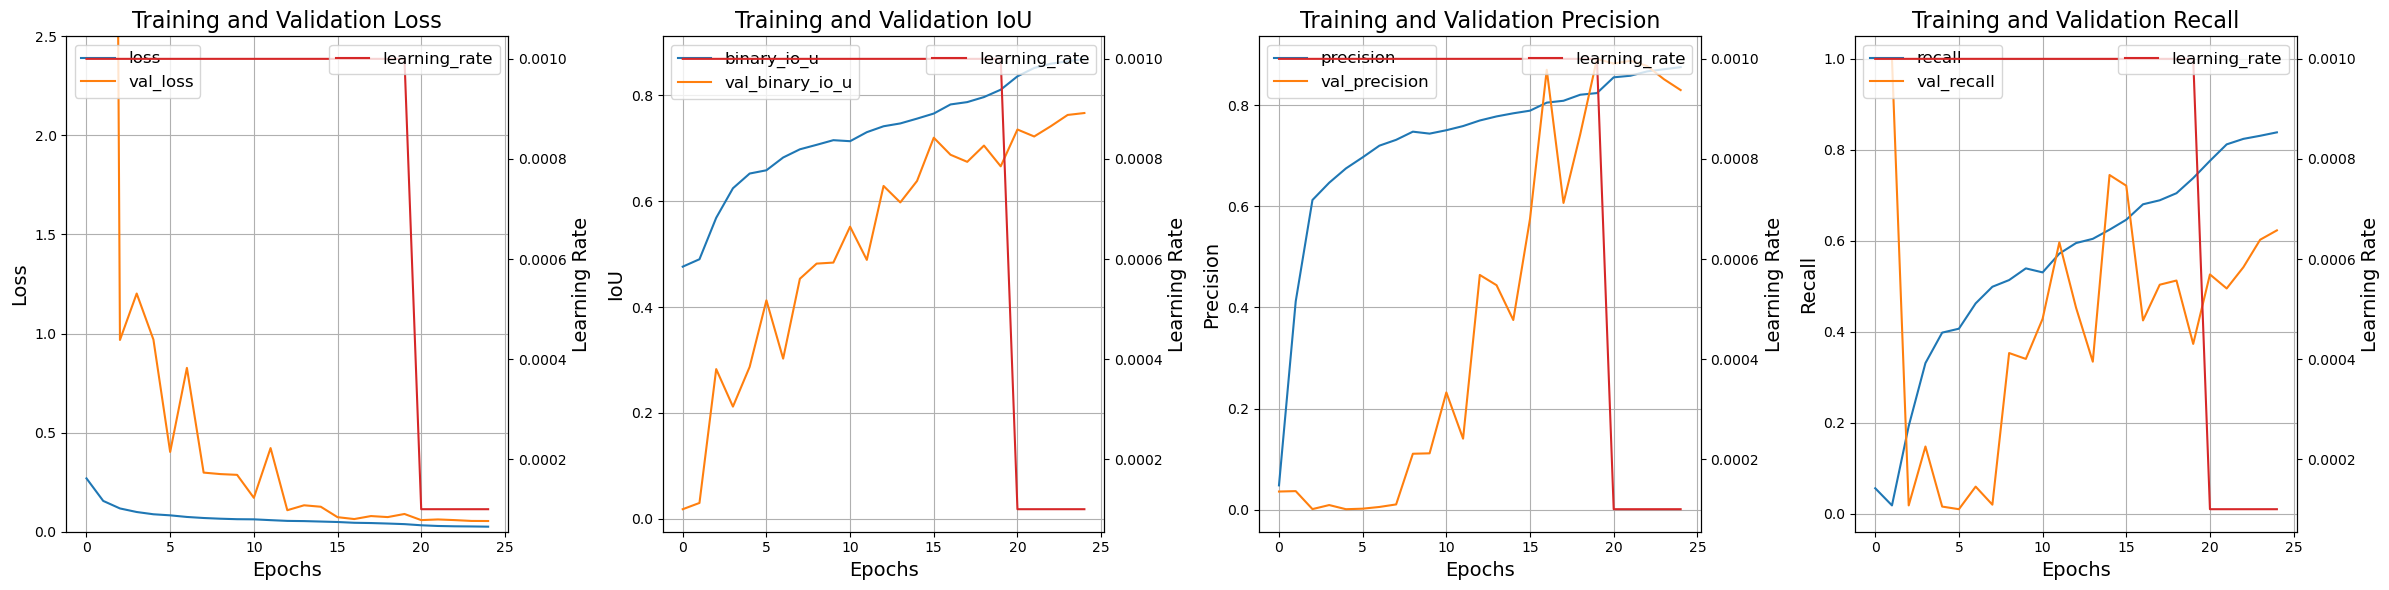
\includegraphics[width=0.8\textwidth]{images/training_sdmodel.png}}\\
  \subfloat{\label{fig:image2}%
      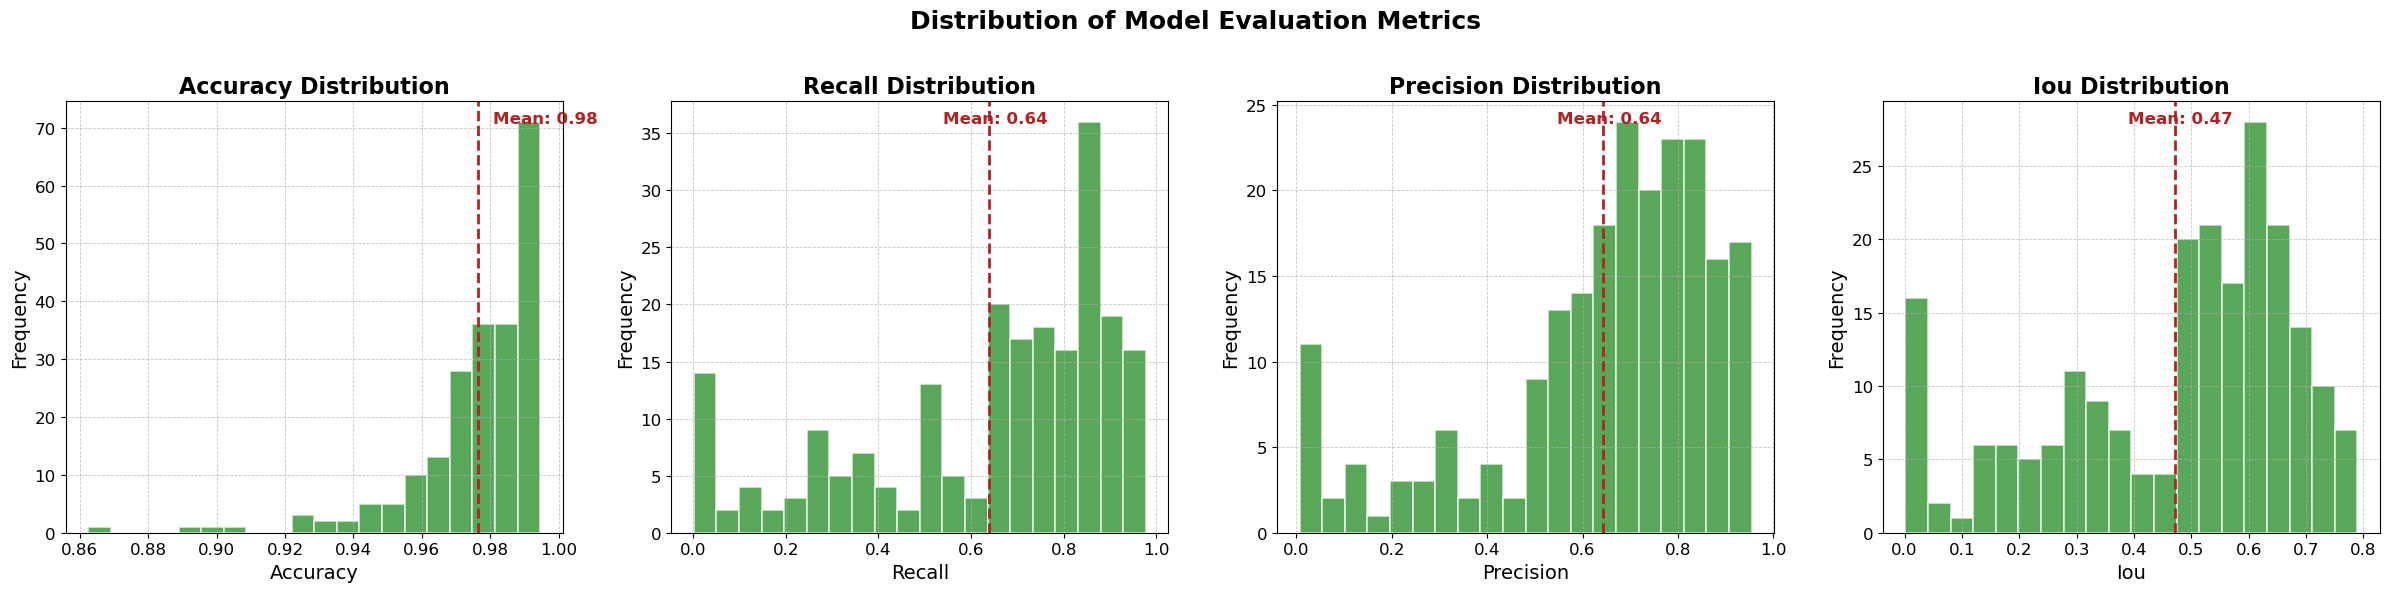
\includegraphics[width=0.8\textwidth]{images/metrics_sdmodel.png}}\\
  \subfloat{\label{fig:image3}%
      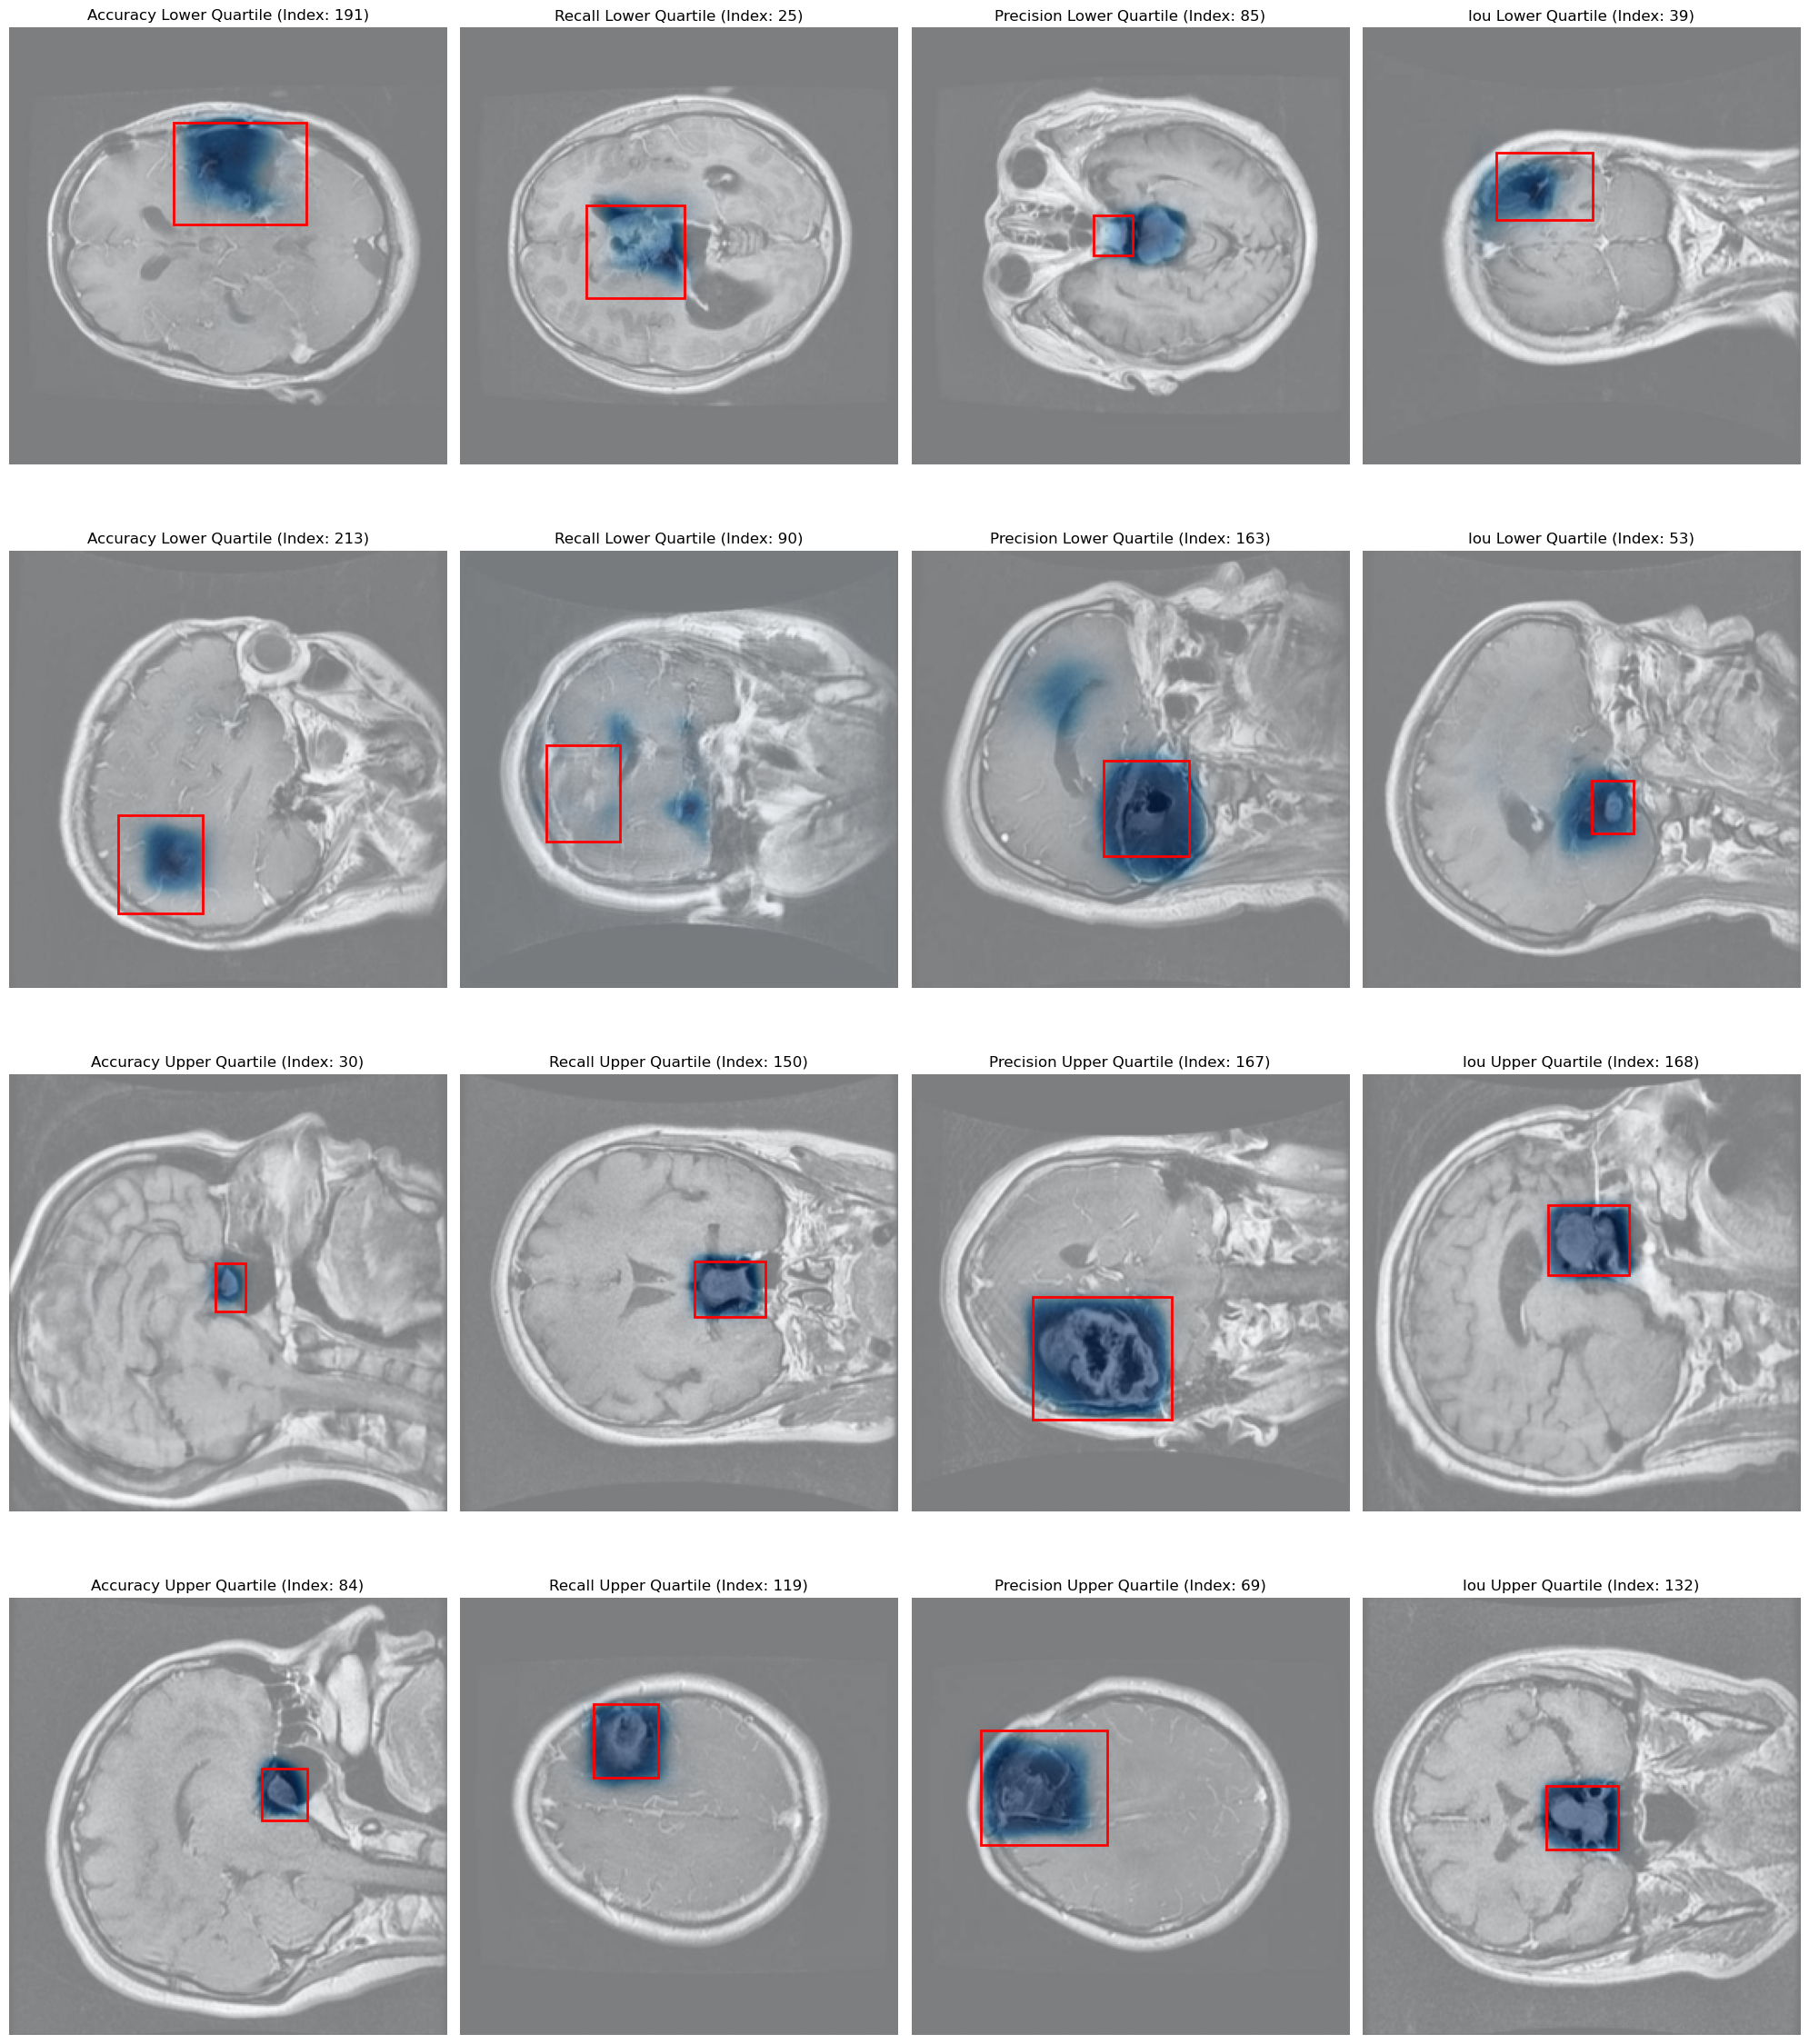
\includegraphics[width=0.7\textwidth]{images/samples_sdmodel.png}}
  \caption{Self-designed model evaluation results: Progress of evaluation metrics during training, result for evaluation metrics per pixel visualized as histograms including the mean as the cumulated accuracy, recall, precision and intersection over union respectively. Additionally two samples for each metric from the upper and lower quartile of the corresponding distribution.}
  \label{fig:eval_sd}
\end{figure*}

\begin{figure*}[h]
  \centering
  \subfloat{\label{fig:image1}%
      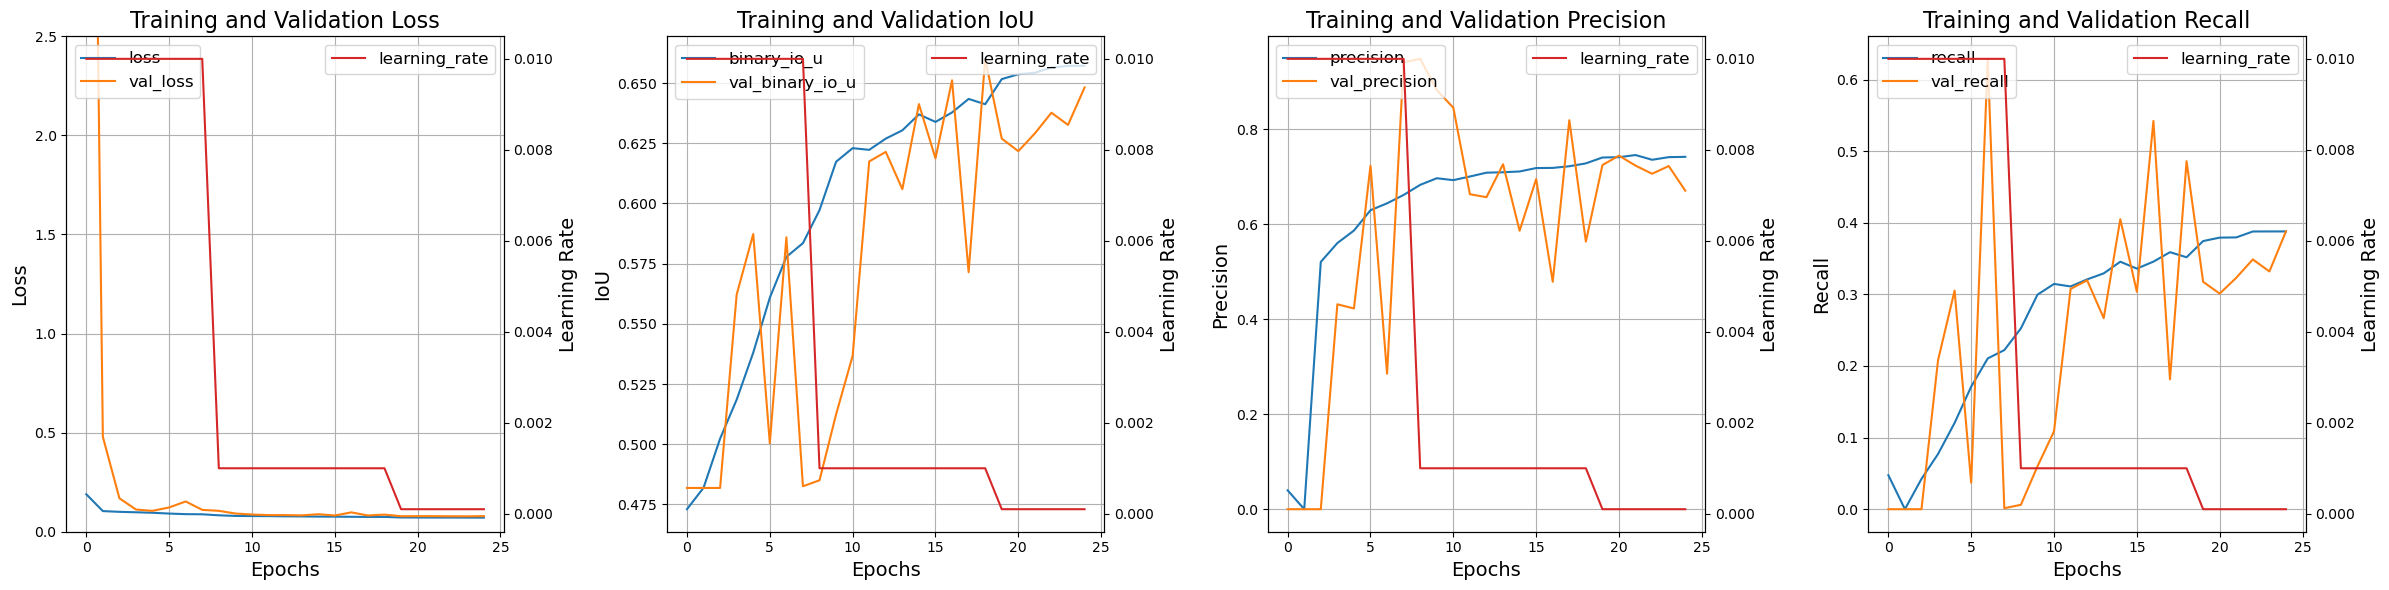
\includegraphics[width=0.8\textwidth]{images/training_ptmodel.png}}\\
  \subfloat{\label{fig:image2}%
      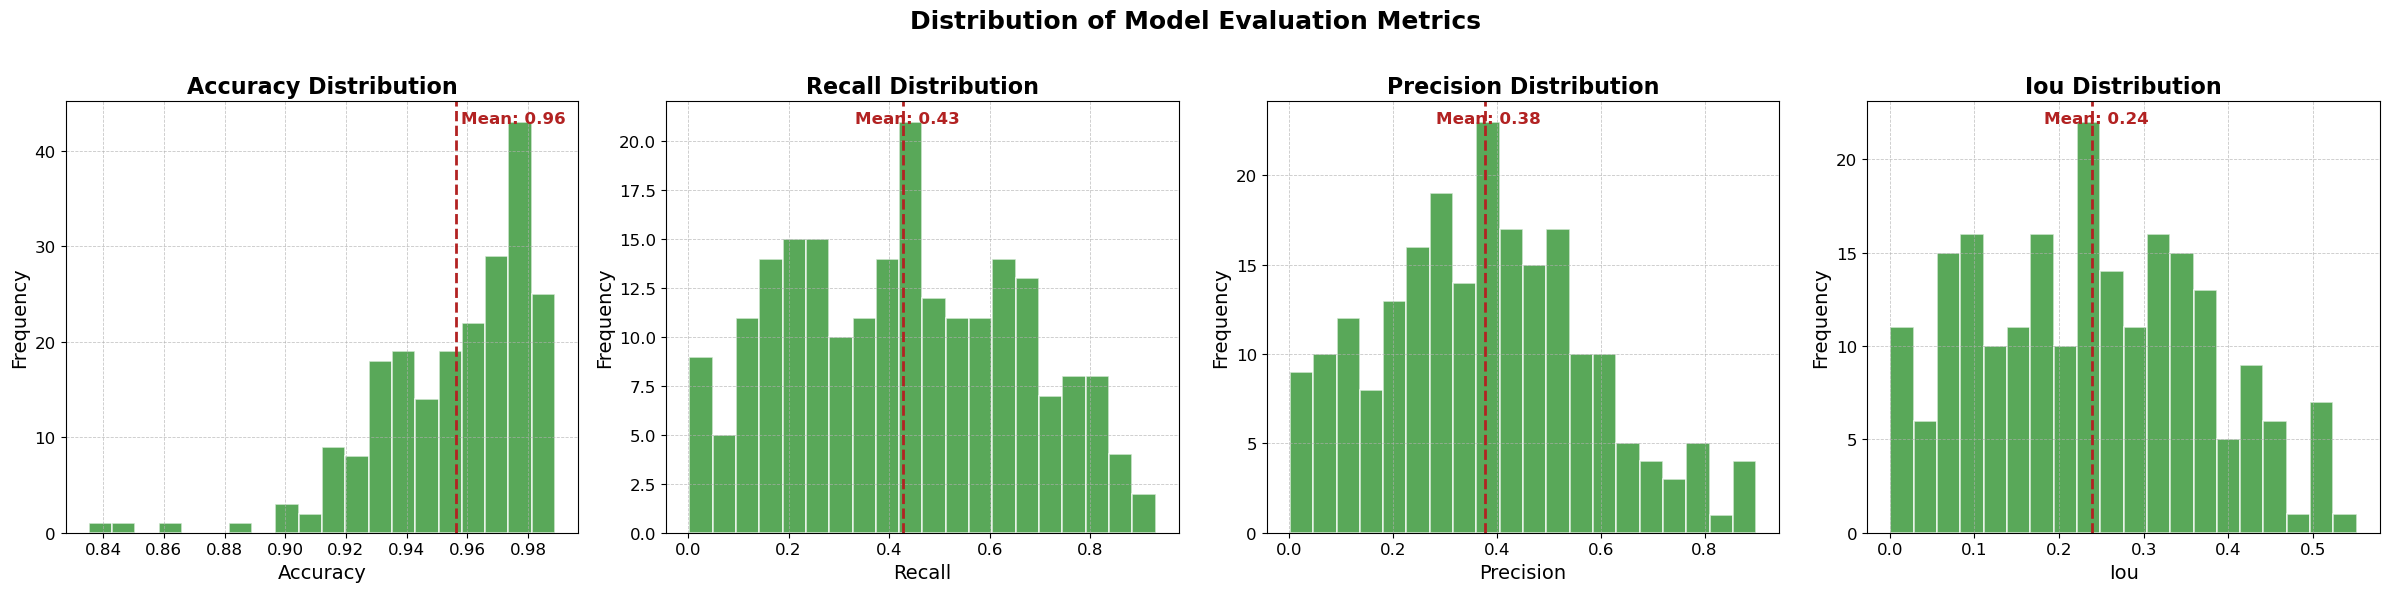
\includegraphics[width=0.8\textwidth]{images/metrics_ptmodel.png}}\\
  \subfloat{\label{fig:image3}%
      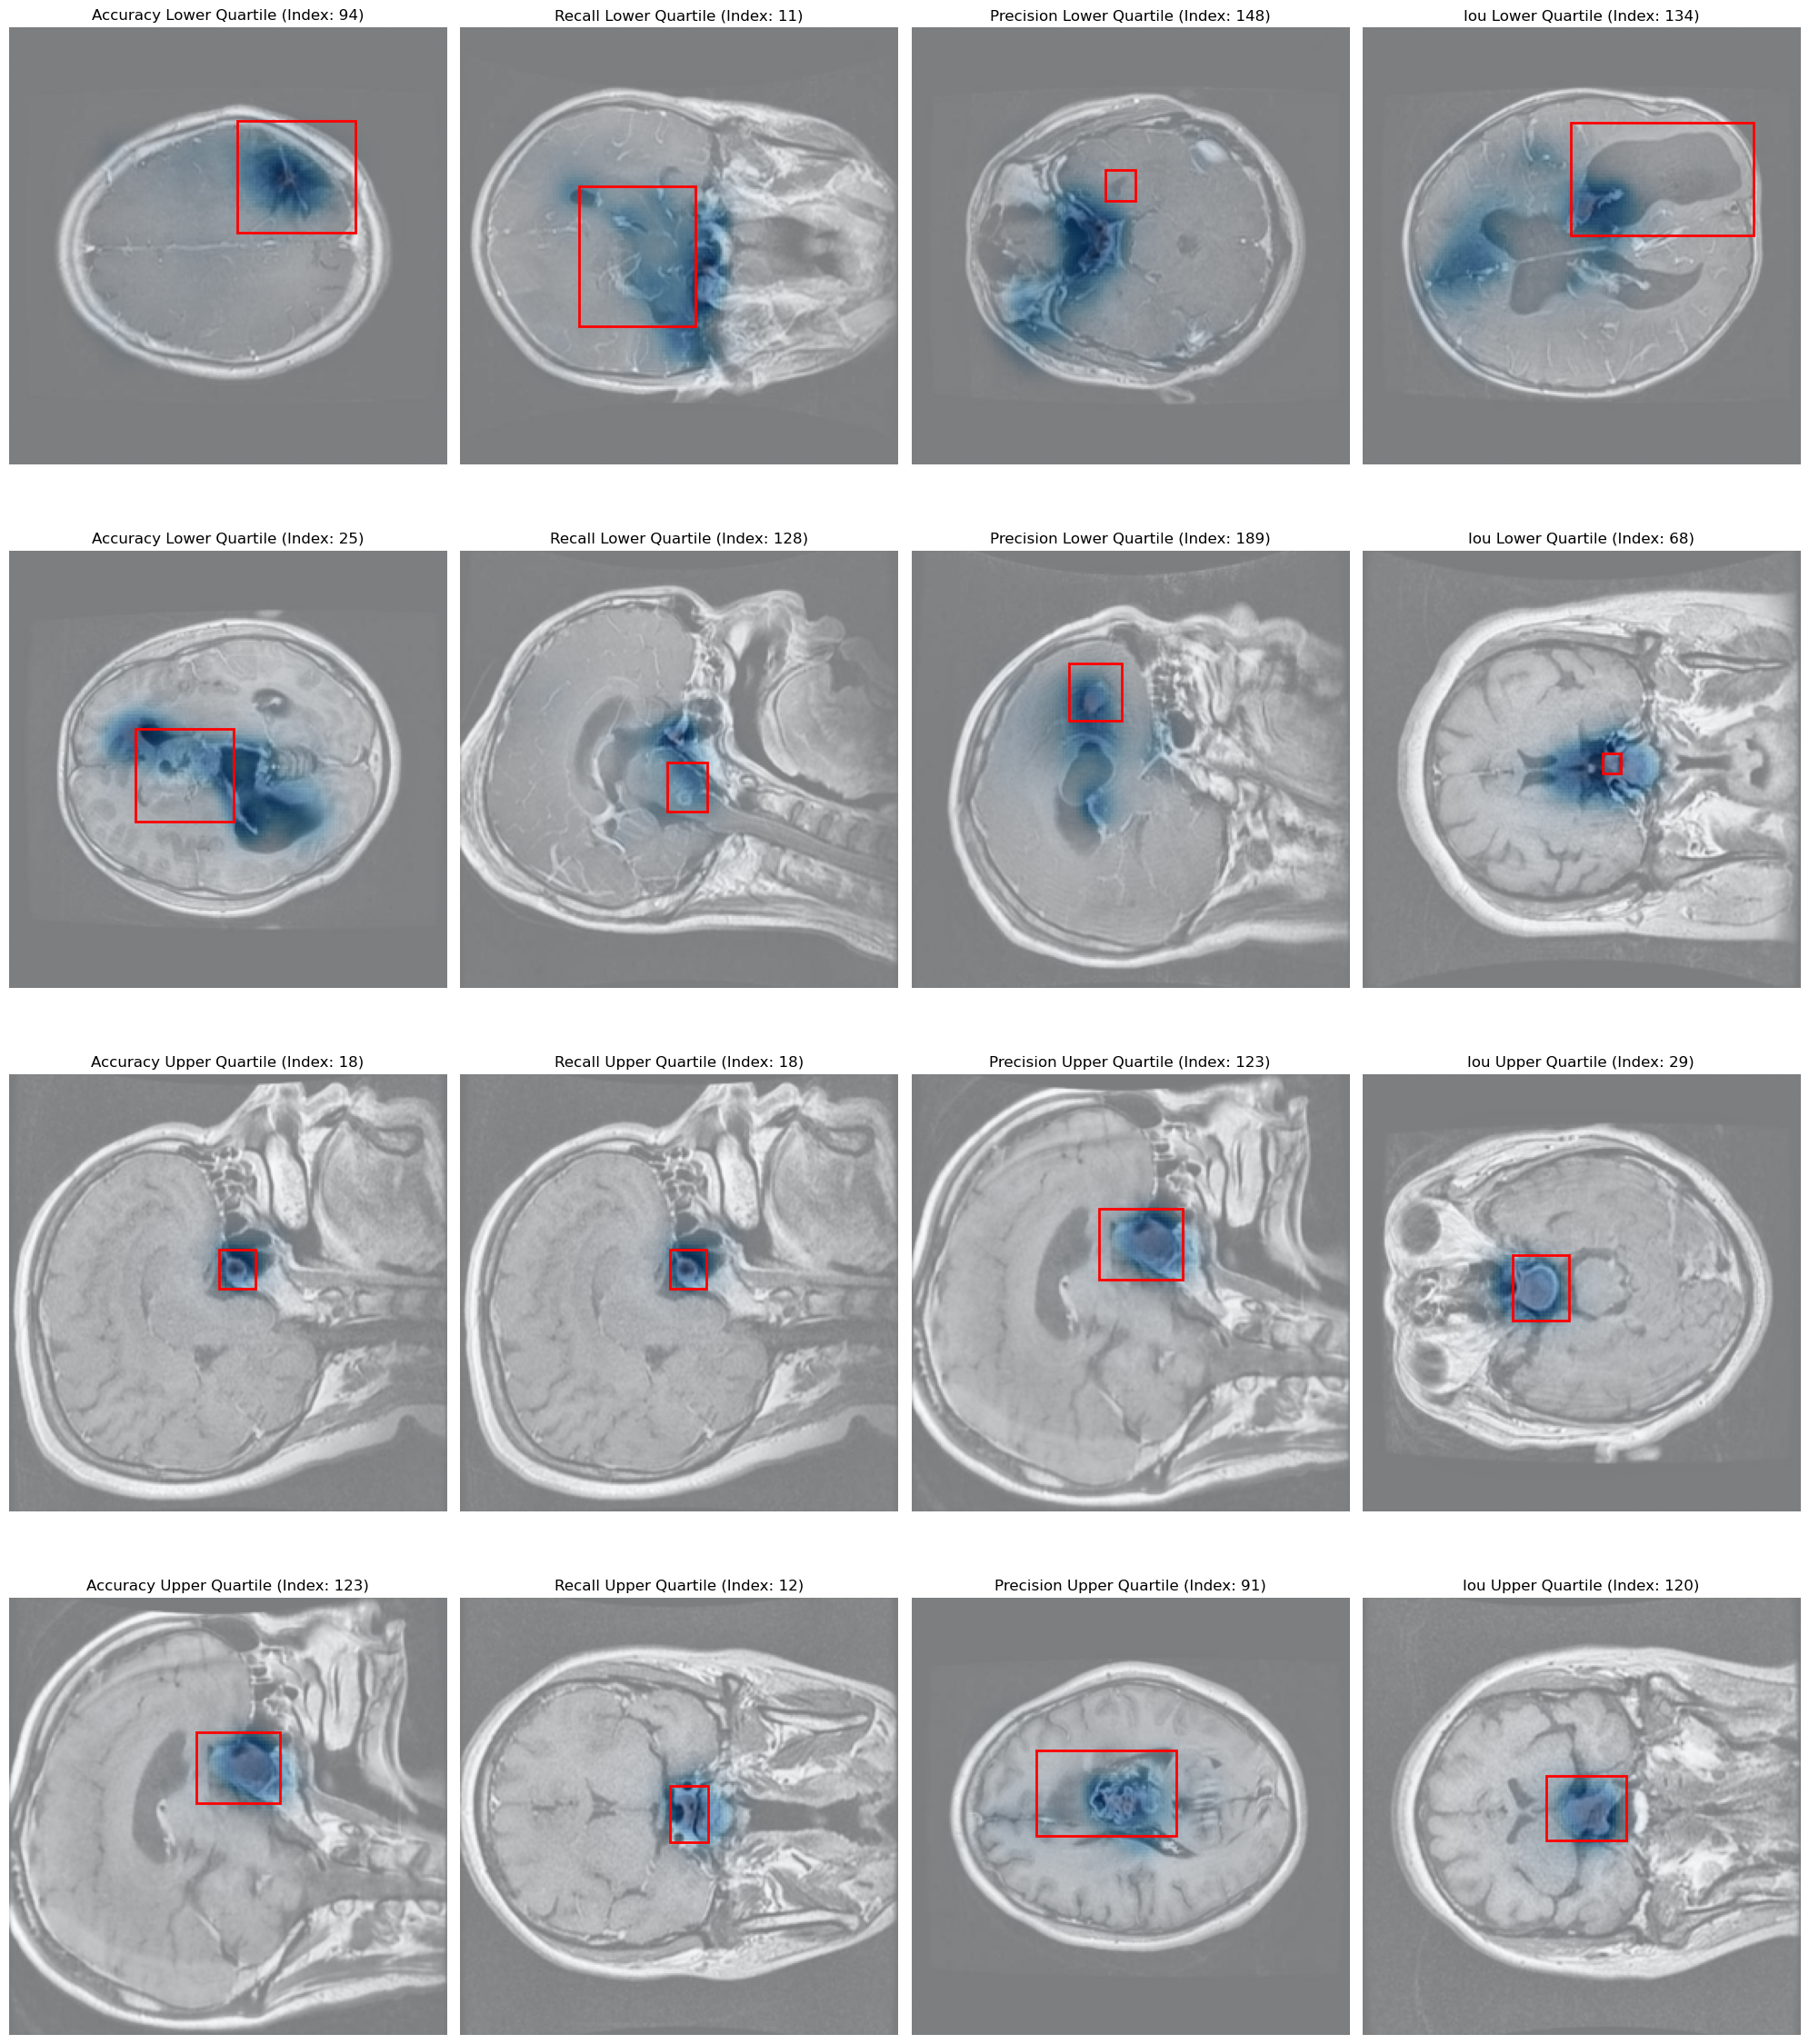
\includegraphics[width=0.7\textwidth]{images/samples_ptmodel.png}}
  \caption{UNet with pretrained ResNet50 Backbone evaluation results: Progress of evaluation metrics during training, result for evaluation metrics per pixel visualized as histograms including the mean as the cumulated accuracy, recall, precision and intersection over union respectively. Additionally two samples for each metric from the upper and lower quartile of the corresponding distribution.}
  \label{fig:eval_pt}
\end{figure*}

\section{Conclusion}
The comparison of the plots indicates that both models improve over the epochs. However, the self-designed model, while showing more variability, eventually trends towards better performance. The plots suggest that longer training could further increase performance. Therefore, this model's architecture might be more optimal for the task of tumor segmentation. At the same time, the self-designed UNET overfits more, possibly due to learning exact features from the training set and struggling to generalize. Adequate tuning of hyperparameters and regularization could improve its performance. Another possibility would be to enhance the training data through image augmentation to facilitate more generalization.
In contrast, the pre-trained model shows superior stability and generalization capability across the metrics, thanks to transfer learning. However, it underperforms, potentially because ResNet50 was trained on a more general task of image classification of different objects. Better results could potentially be achieved through further fine-tuning by unfreezing part or all of the pre-trained weights.

In conclusion, new-trained U-Nets and UNets combining a pre-trained and ResNet50 backnone with a custom head can achieve valuable performance in brain tumor segmentation and.
The application of transfer learning using a combination of a pre-trained ResNet50 based backbone and a UNet head in one model does not improve segmentation performance comparing to an self-designed U-Net model with the same head and the double amount of parameters in the ResNet50 backbone in the given training setup with 25 epochs over the given data set but the evaluation metrics suggest that this kind of models have potential for more consistent and reliable predictions with further training.

Continuing this work, there are a few interesting research questions to follow up. Firtly, an ensemble of both models can be developed and compared to both models to explore possible improvements in the described metrics. Moreover, experimenting with transformer architectures and comparing them with CNNs, an UNets seems to deliver more insights into the capabilities of these architectures. 

\balance

\bibliographystyle{IEEEtran}
\bibliography{bib_CV_MRI_ImSeg}

% \begin{thebibliography}{1} %Example of a Citation: According to a well-known study \cite{ams}, the mathematical typesetting is crucial for clear presentation.

% \bibitem{ams}
% {\it{Mathematics into Type}}, American Mathematical Society. Online available: 

% \bibitem{oxford}
% T.W. Chaundy, P.R. Barrett and C. Batey, {\it{The Printing of Mathematics}}, Oxford University Press. London, 1954.

% \bibitem{lacomp}{\it{The \LaTeX Companion}}, by F. Mittelbach and M. Goossens

% \end{thebibliography}


\end{document}

